Stoffe können sich in den verschiedenen Aggregatzuständen flüssig, fest oder gasförmig
befinden. Diese Zustände sind von zwei Freiheitsgraden abgängig, zum einen der Temperatur $T$,
und zum anderen von dem Druck $p$. Die Abhängigkeit dieser Größen wird klassischerweise
in einem Phasendiagramm dargestellt.

\begin{figure}   % {0.48\textwidth}
  \centering
  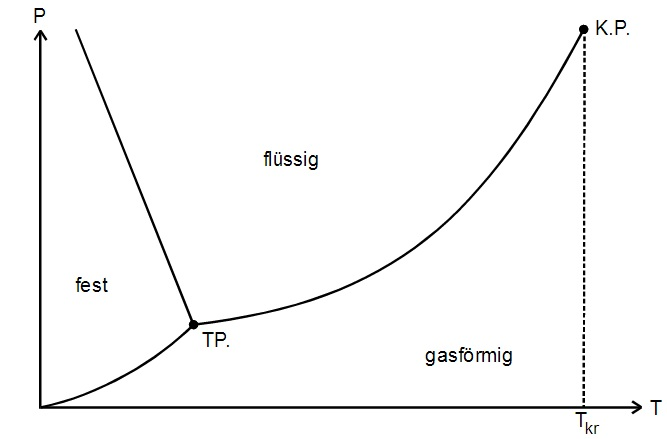
\includegraphics[height=5cm]{Zustandsdiagramm.jpeg}
  \caption{qualitatives Phasendiagramm des Wassers \cite{TU}}
  \label{fig:phase}
\end{figure}

In dem Phasendiagramm ist zu sehen, dass der Druck bei gegebener Temperatur, durch die
Dampfdruckkurve festegelegt ist. Auffällig sind der Tripel-Punkt (T.P.) und
der kritische Punkt (K.P.). Am T.P. liegen alle drei Pahsen vor, am K.P. ist die flüssige
Phase von der gasförmigen Phase nicht mehr zu unterscheiden.
Diese Kurve ist im Wesentlichen von der Verdampfungswärme $L$ abhängig. Sie beschreibt
die Energiemenge, die zur Umwandlung von einem Mol Flüssigkeit in Dampf, gleicher
Temperatur, benötigt wird. Diese Größe $L(T)$ sinkt bei steigender Temperatur und
verschwindet am K.P. ganz \cite{chem}.

Beim Erwärmen der Flüssigkeit erhöht sich die kinetische Energie der Teilchen,
welche nach der Maxwellschen Geschwindigkeitsverteilung bestimmt werden kann. Ist
ihre Energie groß genug, um die Molekular-Kräfte zu überwinden, so können die
Teilchen die Flüssigkeitsoberfläche verlassen und in den gasförmigen Zustand übergehen.
Hierzu muss jedoch entweder Energie von außen hinzugefügt oder dem Wasser entzogen
werden, wodurch dieses abkühlt. Dieser Prozess ist reversibel. Die Verdampfungswärme
wird bei Kondensation somit wieder frei. Zwischen Verdampfung und Kondensation stellt
sich in einem geschlossenem Behältnis nach hinreichend langer Zeit ein Gleichgewicht
ein. Der hier herrschende Druck wird als Sättigungsdampfdruck
bezeichnet. Er hängt nicht vom Volumen des Gasraumes ab, wodurch die allgemeine
Gasgleichung
\begin{equation}
  pV = RT   \ ,\ \text{mit} \ R = \text{allgemeine Gaskonstante} \label{eq:ideal}
\end{equation}
nicht gilt.

Zur Berechnung der Dampfdruckkurve wird der reversible Kreisprozess von Wasser
zwischen Verdampfung und Kondensation betrachtet.

\begin{figure}[H]
  \centering
  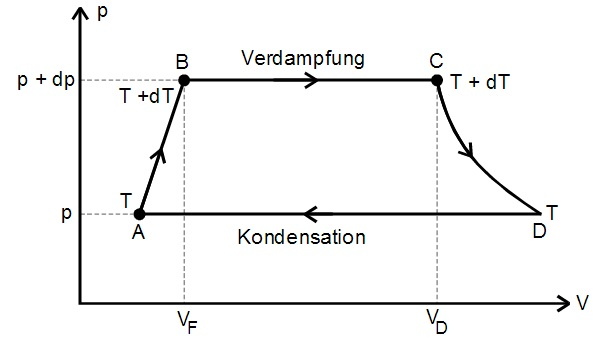
\includegraphics[height=4cm]{Kreisprozess.jpeg}
  \caption{reversibler Kreisprozess für Verdampfung und Kondensation \cite{TU}}
  \label{fig:kreis}
\end{figure}

Zu Beginn ist der Stoff flüssig. Wird nun eine Wärmemenge $dQ$ hinzugefügt,
so erhöht sich der Druck, das Volumen und die Temperatur (A \rightarrow \ B).
Nun verdampft die Flüssigkeit isotherm und isobar, das Volumen
vergrößert sich weiterhin (B \rightarrow \ C). Jetzt kühlt das Gas von der erhöhten
Temperatur wieder ab, wodurch sich auch der Druck senkt (C \rightarrow \ D).
Zuletzt gibt der Dampf die zugeführte Wärmeenergie wieder ab. Dies führt zu einer
isobaren und isothermen Kondensation (D \rightarrow \ A).
Wird nun die geleistete Arbeit mit den Wärmeenergien gleichgesetzt, so ergibt sich
folgende Gleichung:

\begin{equation}
  (C_F - C_D)dT + dL = (_D - V_F)dp .
\end{equation}

Nach dem zweiten Hauptsatz der Thermodynamik folgt für die Summe der Wärmemenge
in einem reversiblen Kreisprozess

\begin{equation}
  \sum_i{\frac{Q_i}{T_i}} = 0 . \notag
\end{equation}

Unter weiteren Vereinfachungen ergibt sich dann die Clausius-Clapeyronsche
Gleichung
\begin{equation}
  (V_D - V_F)dp = \frac{L}{T}dT \label{eq:clausius}.
\end{equation}

Liegt die Temperatur $T$ weit unter der kritischen Temperatur $T_{Kr}$, so können
folgende Näherungen angenommen werden:
\begin{itemize}
  \item $V_F$ ist gegenüber $V_D$ zu vernachlässigen \\
  \item $V_D$ gehorcht der idealen Gasgleichung (\ref{eq:ideal}) \\
  \item $L$ ist druck- und temperaturunabhängig \\
\end{itemize}

Daraus folgt dann

% \qquad für größere Abstände
\begin{align}
  \ln{(p)} &= -\frac{L}{RT} + \ln{(p_0)}  \qquad \text{bzw.} \label{eq:3}  \\
  p &= p_0 \exp{\biggr(-\frac{L}{RT} \biggl)} . \label{eq:4}
\end{align} \cite{TU}
